\documentclass{article}
\usepackage{fancyhdr}
\usepackage{amsmath,amssymb}
\usepackage{geometry}
\usepackage{datetime}
\usepackage{enumerate}
\usepackage{graphicx}

%Insert page formatting here
\hoffset = -.5in
\voffset = -0.375in
\textwidth = 7in
\textheight = 9in
\headheight = 24pt

\pagestyle{fancy}

\rhead{Peter Olson\\Student ID: $441666$}
\lhead{Math 3200\\Homework 10}
\chead{\today}
\cfoot{}

%\addtolength{\headwidth}{\marginparsep}
%\addtolength{\headwidth}{\marginparwidth}

%\renewcommand{\labelitemi}{$\diamond$}
\renewcommand{\implies}{\rightarrow}
\newcommand{\widespace}{\qquad \qquad \;}
\newcommand{\tret}{\\ \hline}
\newcommand{\fh}{\tfrac{1}{2}}
\newcommand{\deriv}[2]{\frac{d #1}{d #2}}
\newcommand{\pderiv}[2]{\frac{\delta #1}{\delta #2}}
\newcommand{\vr}{\vec{r}}
\newcommand{\at}{\text{ at }}
\newcommand{\var}{\text{Var}}
\newcommand{\cov}{\text{Cov}}

\begin{document}

\section*{Exercise 10.6}

\begin{enumerate}[\quad(a)]
	\item Make a scatter plot for the boiling point by barometric pressure. Does the relationship appear to be approximately linear?\\
	\begin{center}
		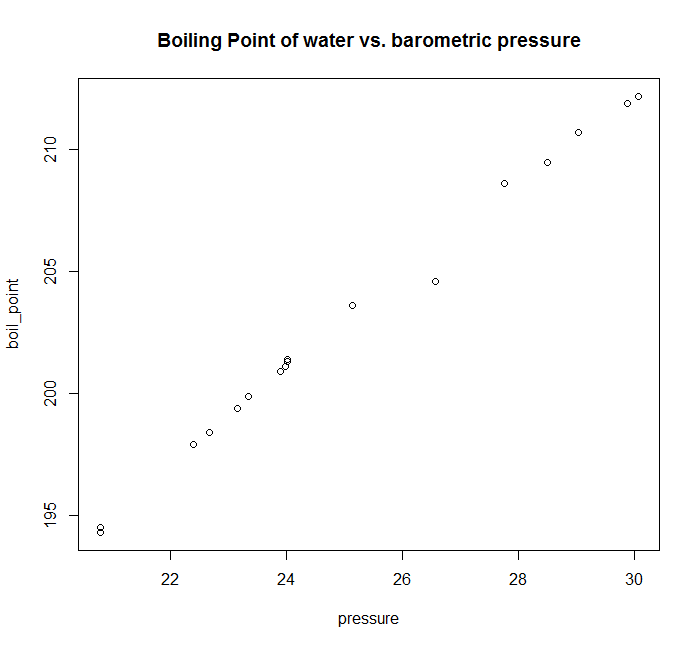
\includegraphics[width=3.5in]{Q41.png}
	\end{center}
	The relationship appears very much linear.
	\item Fit a least squares regression line. What proportion of variation in the boiling point is accounted for by linear regression on the barometric pressure?\\
	\begin{center}
		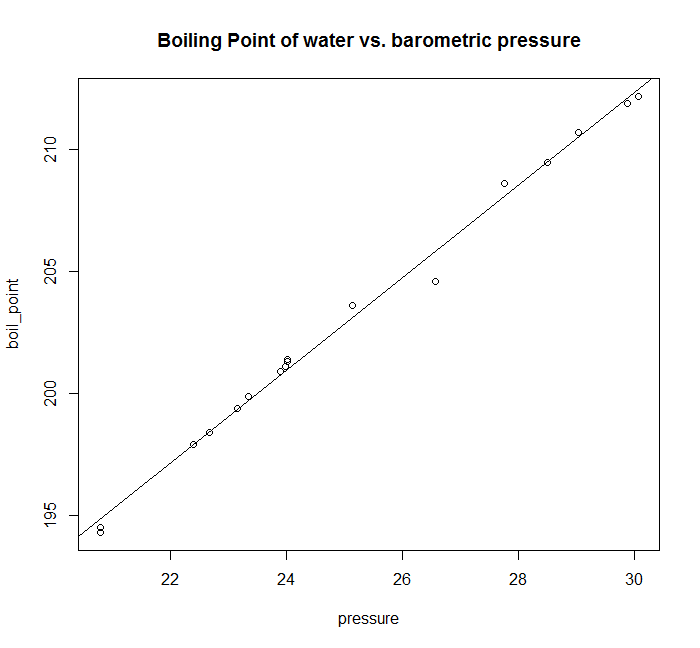
\includegraphics[width=3.5in]{Q42.png}
	\end{center}

	The $r^2$ value from the fit is \texttt{0.9944}
	\newpage
	\item Calculate the mean square error estimate of $\sigma$.

	$\sigma =$ \texttt{0.4440}
\end{enumerate}

\section*{Exercise 10.10 + (c)}

\begin{enumerate}[\quad(a)]
	\item Calculate a 95\% CI for the boiling point if the barometric pressure is 28 inches of mercury. Interpret your CI.

	95\% confidence interval $\rightarrow\ [208.537, 208.556]$
	
	Because there's such a strong linear correlation in the data and this point is within the range of the data, the confidence interval is very, very small, with $\pm 0.01$ of the mean on either side.
	\item Calculate a 95\% CI for the boiling point if the barometric pressure is 31 inches of mercury. Compare this with the CI of (a).

	95\% confidence interval $\rightarrow\ [215.236, 214.267]$

	This confidence interval is much larger than that of part (a) because it's actually beyond the range of the data.
	\item Calculate a 95\% PI for the boiling point at the pressure of 31 inches of mercury. Compare this with the CI in (b) and explain the difference.

	95\% prediction interval $\rightarrow\ [214.220, 214.284]$

	While the confidence interval is concerned with estimating $y$ given $x$, the prediction interval takes into account an additional error term, and has a wider spread than the confidence. Prediction intervals, after all, have to anticipate the performance of a particular individual measurement, not just the average statistic.
\end{enumerate}

\end{document}